\documentclass[a4paper, 12pt]{article}
\usepackage[utf8]{inputenc}

\usepackage[a4paper,top=1.3cm,bottom=2cm,left=1.5cm,right=1.5cm,marginparwidth=0.75cm]{geometry}
\usepackage{cmap}				
\usepackage{mathtext} 				
\usepackage[T2A]{fontenc}			
\usepackage[utf8]{inputenc}			
\usepackage[english,russian]{babel}	
\usepackage{multirow}
\usepackage{mathtools}
\mathtoolsset{showonlyrefs=true}

\usepackage{graphicx}
\usepackage{wrapfig}
\usepackage{tabularx}

\usepackage{pgfplots}
\pgfplotsset{compat=1.9}

\title{2.1.3-theory}
\author{Влад Черниенко}
\date{March 2022}

\begin{document}
    
    \begin{titlepage}
    
        \begin{center}
                {\large МОСКОВСКИЙ ФИЗИКО-ТЕХНИЧЕСКИЙ ИНСТИТУТ (НАЦИОНАЛЬНЫЙ ИССЛЕДОВАТЕЛЬСКИЙ УНИВЕРСИТЕТ)}
            \end{center}
            \begin{center}
                {\large Фихтех-школа радиотехники и компьютерных технологий}
            \end{center}
            
            \vspace{4.5cm}
            
            {\huge
                \begin{center}
                    {\bf Лабораторная работа 2.1.3}\\
                    Определение $ C_{p}/C_{v} $ по скорости звука в газе
                \end{center}
            }
            
            \vspace{12cm}
            
            \begin{flushright}
                {\LARGE Автор: \\ Черниенко Владислав Антонович \\ \vspace{0.2cm} Группа Б01-110}
            \end{flushright}
    
    \end{titlepage}
 
 
    \noindent {\bf Цель работы:} 1) измерение частоты колебаний и длины волны при резонансе звуковых колебаний в газе, заполняющем трубу; 2) определение показателя адиабаты с помощью уравнения состояния идеального газа.\\
    
    \noindent{\bf В работе используются:} звуковой генератор ГЗ; электронный осциллограф ЭО; микрофон; телефон; раздвижная труба; теплоизолированная труба, обогреваемая водой из термостата; баллон со сжатым углекислым газом; газгольдер.\\
   
    \begin{flushleft}
        {\Large {\bf Теоретические сведения}}
    \end{flushleft}
    
    Скорость распространения звуковой волны в газах зависит от показателя адиабаты $ \gamma $. На измерении скорости звука основан один из наиболее точных методов определения показателя адиабаты
    
    Скорость звука в газах определяется формулой:
    \begin{equation}
        c=\sqrt{\gamma\frac{RT}{\mu}},
    \end{equation}
    \noindent где $ R $ — газовая постоянная, $ T $ — температура газа, а $ \mu $ — его молярная масса. Преобразуя эту формулу, найдём
    \begin{equation}
        \gamma=\frac{\mu}{RT}c^{2}.
        \label{first}
    \end{equation}
    \noindent Таким образом, для определения показателя адиабаты достаточно измерить температуру газа и скорость распространения звука (молярная масса газа предполагается известной).
    
    Звуковая волна, распространяющаяся вдоль трубы, испытывает многократные отражения от торцов. Звуковые колебания в трубе являются наложением всех отражённых волн и, вообще говоря, очень сложны. Картина упрощается, если длина трубы $ L $ равна целому числу полуволн, то есть когда
    \begin{equation}
        L=n\frac{\lambda}{2},
        \label{second}
    \end{equation}
    \noindent где $ \lambda $ — длина волны звука в трубе, а $ n $ — любое целое число. Если условие \eqref{second} выполнено, то волна, отражённая от торца трубы, вернувшаяся к её началу и вновь отражённая, совпадает по фазе с падающей. Совпадающие по фазе волны усиливают друг друга. Амплитуда звуковых колебаний при этом резко возрастает — наступает резонанс.
    
    Скорость звука связана с его частотой $ f $ и длиной волны $ \lambda $ соотношением
    \begin{equation}
        c=\lambda f.
        \label{third}
    \end{equation}
    
    При постоянной длине трубы можно изменять частоту звуковых колебаний. В этом случае следует плавно изменять частоту $ f $ звукового генератора, а следовательно, и длину звуковой волны $ \lambda $. Для последовательных резонансов получим
    \begin{equation}
        L=\frac{\lambda_{1}}{2}n=\frac{\lambda_{2}}{2}(n+1)=...=\frac{\lambda_{k+1}}{2}(n+k).
        \label{fourth}
    \end{equation}
    Из \eqref{third} и \eqref{fourth} имеем
    \begin{equation}
        f_{1}=\frac{c}{\lambda_{1}}=\frac{c}{2L}n,\hspace{0.5cm}
        f_{2}=\frac{c}{\lambda_{2}}=\frac{c}{2L}(n+1)=f_{1}+\frac{c}{2L},\hspace{0.2cm}
        ...,\hspace{0.5cm}
        f_{k+1}=\frac{c}{\lambda_{k+1}}=\frac{c}{2L}(n+k)=f_{1}+\frac{c}{2L}k.
        \label{fifth}
    \end{equation}
    Скорость звука, деленная на $ 2L $, определяется, таким образом, по угловому коэффициенту графика зависимости частоты от номера резонанса.\\
    
    \begin{flushleft}
        {\Large {\bf Экспериментальная установка}}
    \end{flushleft}
    
    В установке (рис. \ref{pic1}) звуковые колебания в трубе возбуждаются телефоном Т и улавливаются микрофоном М. Мембрана телефона приводится в движение переменным током звуковой частоты; в качестве источника переменной ЭДС используется звуковой генератор ГЗ. Возникающий в микрофоне сигнал наблюдается на осциллографе ЭО.
    
    Микрофон и телефон присоединены к установке через тонкие резиновые трубки. Такая связь достаточна для возбуждения и обнаружения звуковых колебаний в трубе и в то же время мало возмущает эти колебания: при расчётах оба торца трубы можно считать неподвижными, а влиянием соединительных отверстий пренебречь.
    
    Установка содержит теплоизолированную трубу постоянной длины. Воздух в трубе нагревается водой из термостата. Температура газа принимается равной температуре воды, омывающей трубу. На этой установке измеряется зависимость скорости звука от температуры.\\
    
    \begin{figure}[ht]
        \center{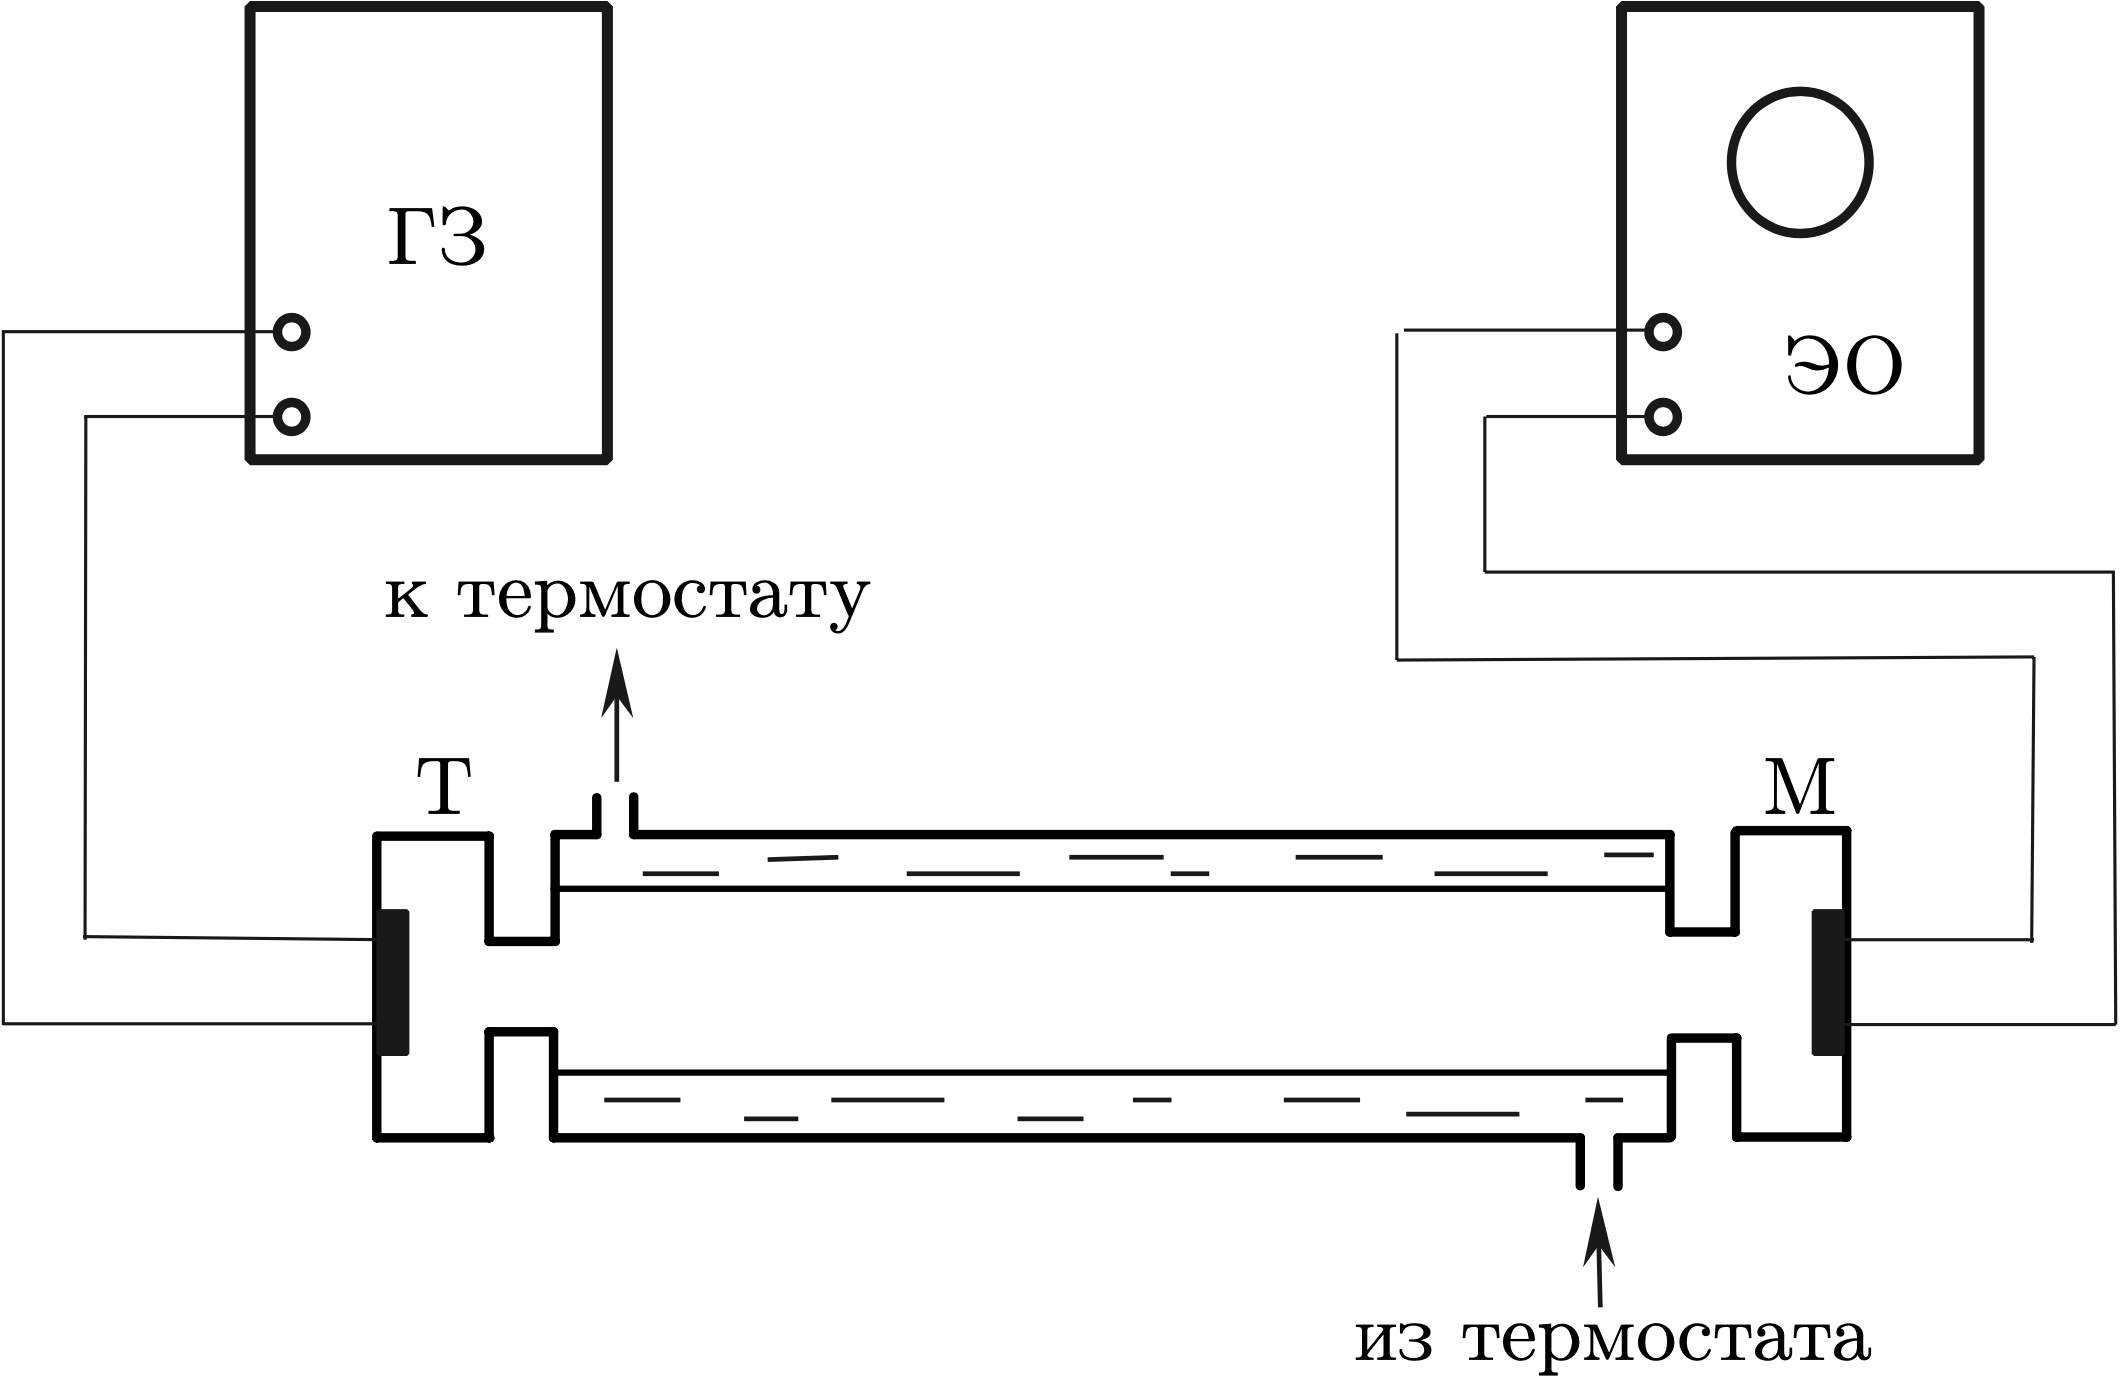
\includegraphics[width=30pc]{ust1.png}}
        \caption{Установка для изучения зависимости скорости звука от температуры}
        \label{pic1}
    \end{figure}
    
    \begin{flushleft}
        {\Large {\bf Ход работы}}
    \end{flushleft}
    
    \begin{enumerate}
    
        \item[1.] Запишем значения комнатной температуры и длины используемой трубы:
        \begin{equation}
            T_{к} = 21,9^{\circ}  C, \text{ } L = (800\pm1) \text{ мм}.
        \end{equation}
        
        \item[2.] Включим электронный осцилограф ЭО и звуковой генератор ГЗ и дадим им прогреться 5-7 минут. Включим на осцилографе тумблер «луч» и ручками управления добьёмся прямой линии на экране. Установим нуль на звуковом генераторе.
        
        \item[3.] Подберём напряжение на выходе генератора так, чтобы при резонансе на осциллографе наблюдались колебания достаточной амплитуды.
        
        \item[4.] Посчитаем погрешность измерений частот: $\sigma_f = 6 \text{ Гц}$.
        
        \item[5.] Примем скорость звука в воздухе при комнатной температуре равной табличному значению $ c_{табл} = 343 \text{ }\frac{\text{м}}{\text{с}} $ и оценим значение частоты для первого резонанса по формуле \eqref{third}:
        \begin{equation}
            f_{оц} = \frac{c_{табл}}{2L} = \frac{343}{1,6} = 214,3 \text{ Гц}.
        \end{equation}
        
        \item[6.] Плавно увеличивая частоту генератора, получим ряд последовательных резонансых значений частоты. Результаты будем заносить в табл. \ref{table1}.
        
        \item[7.] Включим термостат и настроим его на температуру $25^{\circ}C$. повторим измерения п. 5 при данном значении температуры. Результаты занесём в табл. \ref{table1}.
        
        \item[8.] Будем повышать температуру на $\Delta T = 2^{\circ}C$ до $48^{\circ}C$. Для каждого значения температуры повторим измерения п. 5. Результаты будем вносить в табл. \ref{table1}.
        
        \item[9.] При последнем измерении резонансных частот измерим действительное значение температуры трубы и сравним его со значением на термостате:
        \begin{equation}
            \sigma_{T} = T_{посл} - T_{трубы} = 4,7^{\circ}C.
        \end{equation}
         
    \end{enumerate}
    
    \begin{table}[ht]
        \centering
        \begin{tabular}{|c|c|c|c|c|c|c|c|c|c|c|c|}
            \hline
            $T$, К & $k$ & $f_{k+1}$, Гц & $T$, К & $k$ & $f_{k+1}$, Гц & $T$, К & $k$ & $f_{k+1}$, Гц & $T$, К & $k$ & $f_{k+1}$, Гц \\
            \hline
            \multirow{5}*{294,9} & 0 & 206 & \multirow{5}*{298} & 0 & 206,5 & \multirow{5}*{300,1} & 0 & 203,4 & \multirow{5}*{302,1} & 0 & 204,7 \\
            \cline{2-3}\cline{5-6}\cline{8-9}\cline{11-12}
             & 2 & 659 & & 2 & 660,7 & & 2 & 662,3 & & 2 & 664,4 \\
            \cline{2-3}\cline{5-6}\cline{8-9}\cline{11-12}
             & 4 & 1086 & & 4 & 1089,4 & & 4 & 1091,7 & & 4 & 1095,3 \\
            \cline{2-3}\cline{5-6}\cline{8-9}\cline{11-12}
             & 6 & 1518 & & 6 & 1522,9 & & 6 & 1526,2 & & 6 & 1531,8 \\
            \cline{2-3}\cline{5-6}\cline{8-9}\cline{11-12}
             & 8 & 1949 & & 8 & 1956,8 & & 8 & 1961,2 & & 8 & 1967,1 \\
            \hline
            \multirow{5}*{305,2} & 0 & 204,3 & \multirow{5}*{306,9} & 0 & 204,6 & \multirow{5}*{308,9} & 0 & 204,6 & \multirow{5}*{311} & 0 & 204,9 \\
            \cline{2-3}\cline{5-6}\cline{8-9}\cline{11-12}
             & 2 & 665,9 & & 2 & 669,4 & & 2 & 669,8 & & 2 & 671,6 \\
            \cline{2-3}\cline{5-6}\cline{8-9}\cline{11-12}
             & 4 & 1098,9 & & 4 & 1103,6 & & 4 & 1105,1 & & 4 & 1107,2 \\
            \cline{2-3}\cline{5-6}\cline{8-9}\cline{11-12}
             & 6 & 1536,7 & & 6 & 1543,1 & & 6 & 1545 & & 6 & 1548,6 \\
            \cline{2-3}\cline{5-6}\cline{8-9}\cline{11-12}
             & 8 & 1973 & & 8 & 1981,6 & & 8 & 1984,2 & & 8 & 1988,9 \\
            \hline
            \multirow{5}*{313,1} & 0 & 205,8 & \multirow{5}*{315,1} & 0 & 207,1 & \multirow{5}*{317} & 0 & 206,8 & \multirow{5}*{319,1} & 0 & 205,5 \\
            \cline{2-3}\cline{5-6}\cline{8-9}\cline{11-12}
             & 2 & 672,4 & & 2 & 674,8 & & 2 & 676,3 & & 2 & 677,3 \\
            \cline{2-3}\cline{5-6}\cline{8-9}\cline{11-12}
             & 4 & 1109,1 & & 4 & 1112,9 & & 4 & 1115 & & 4 & 1117,2 \\
            \cline{2-3}\cline{5-6}\cline{8-9}\cline{11-12}
             & 6 & 1551,2 & & 6 & 1556,3 & & 6 & 1559,8 & & 6 & 1562,3 \\
            \cline{2-3}\cline{5-6}\cline{8-9}\cline{11-12}
             & 8 & 1992,6 & & 8 & 1998,3 & & 8 & 2002,8 & & 8 & 2006,7 \\
            \hline
            \multirow{5}*{321} & 0 & 207,2 \\
            \cline{2-3}
             & 2 & 679,4 \\
            \cline{2-3}
             & 4 & 1120,1 \\
            \cline{2-3}
             & 6 & 1566,8 \\
            \cline{2-3}
             & 8 & 2012,1 \\
            \cline{1-3}
        \end{tabular}
        \caption{Резонансые значения частоты звуковой волны для различных температур}
        \label{table1}
    \end{table}
    
    \begin{flushleft}
        {\Large {\bf Обработка результатов измерений}}
    \end{flushleft}
    
    \begin{enumerate}
    
        \item[1.] Проведём наилучшие прямые через точки зависимости номера резонанса $k$ и разницы частоты при данном резонансе $f_{k+1}$ и частоты при $k=0$, т.е. $f_1$ при данных температурах. Результаты приведены на рис. \ref{pic2}.
        
        \begin{figure}[ph]
            \begin{minipage}[h]{0.5\linewidth}
                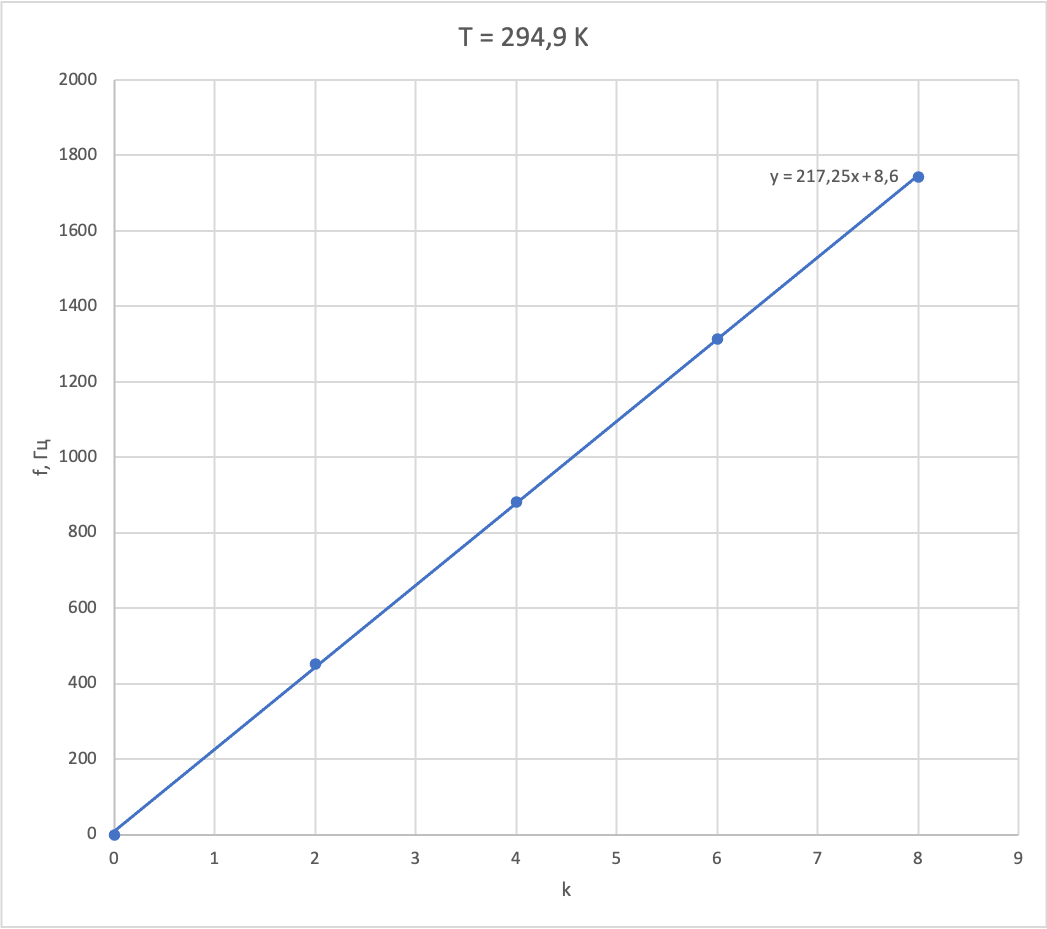
\includegraphics[width=1\linewidth]{1.png}
            \end{minipage}
            \hfill
            \begin{minipage}[h]{0.5\linewidth}
                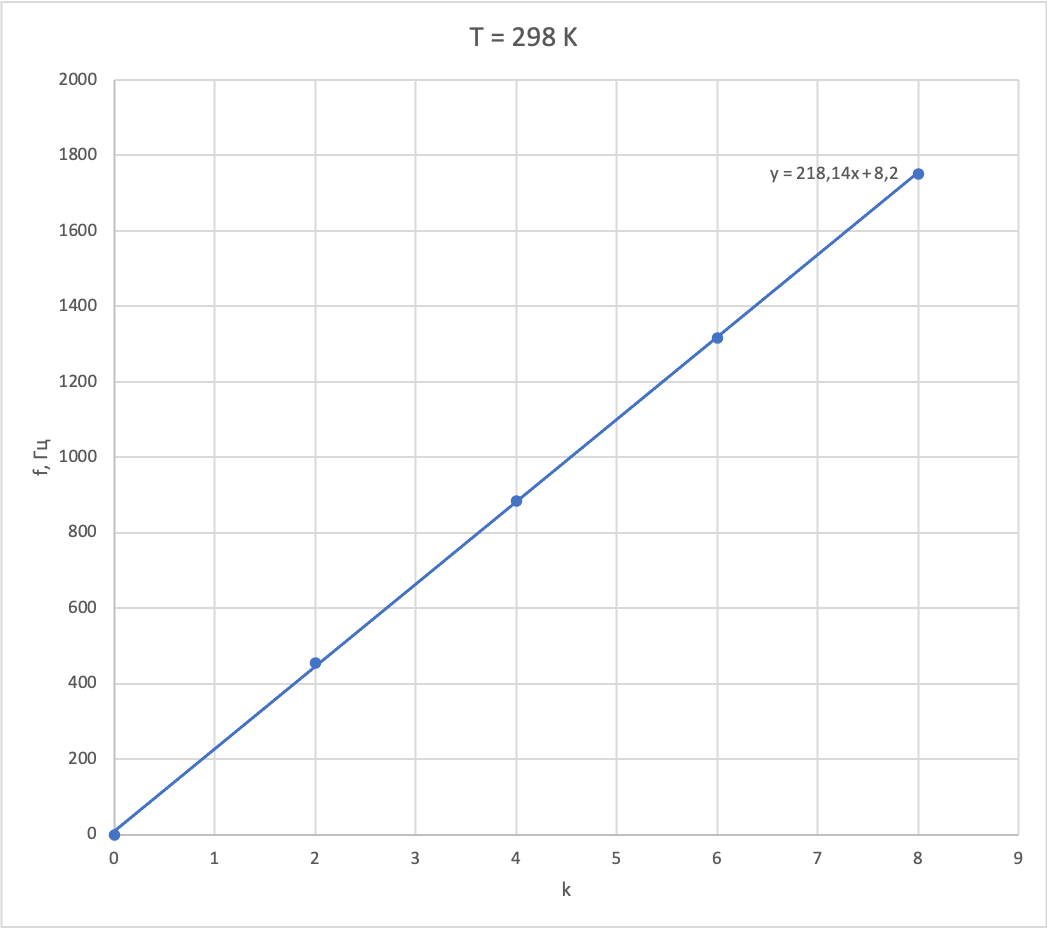
\includegraphics[width=1\linewidth]{2.png}
            \end{minipage}
            \vfill
            \begin{minipage}[h]{0.5\linewidth}
                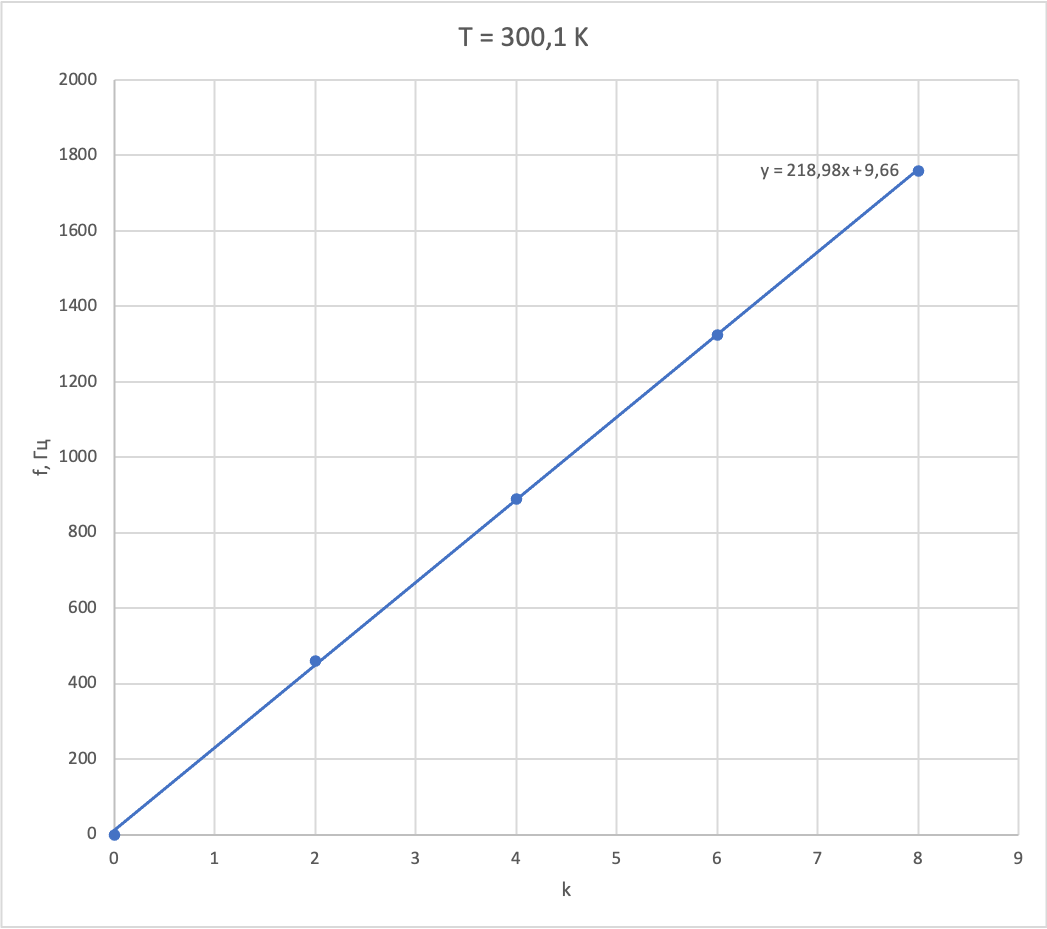
\includegraphics[width=1\linewidth]{3.png}
            \end{minipage}
            \hfill
            \begin{minipage}[h]{0.5\linewidth}
                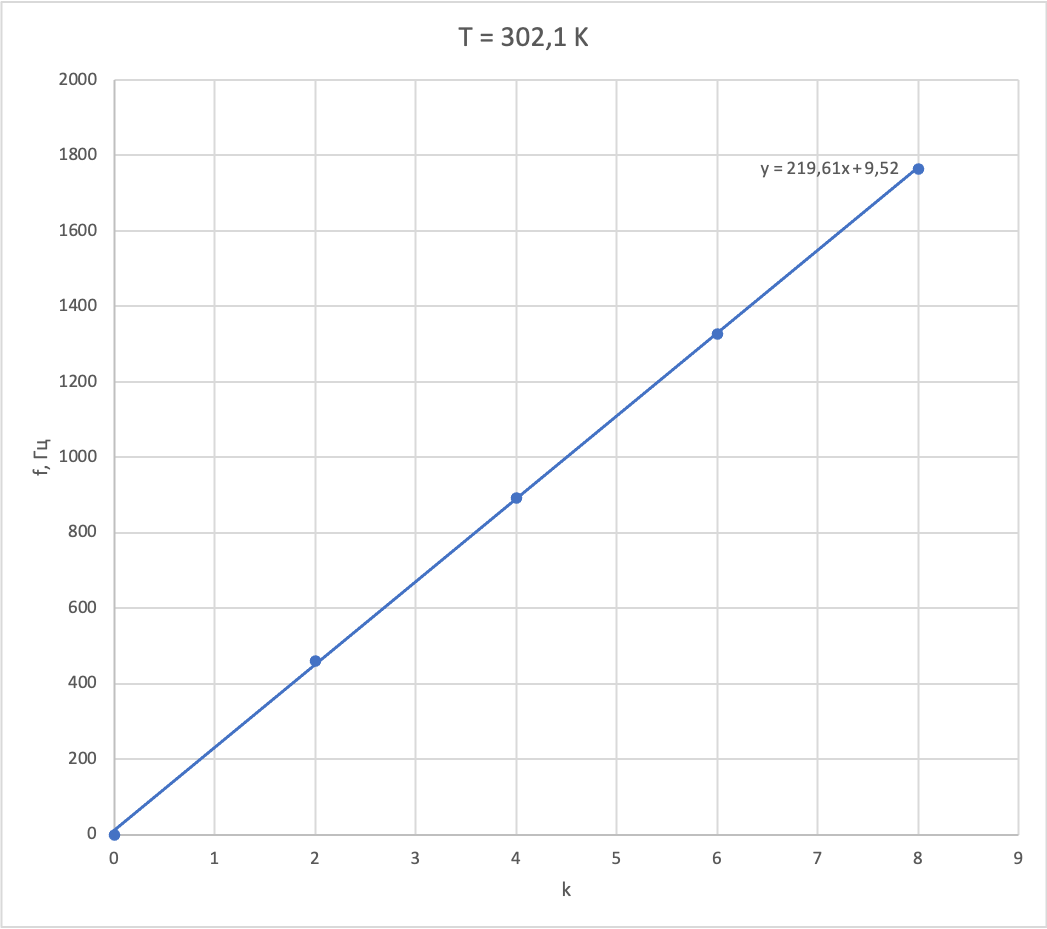
\includegraphics[width=1\linewidth]{4.png}
            \end{minipage}
            \vfill
            \begin{minipage}[h]{0.5\linewidth}
                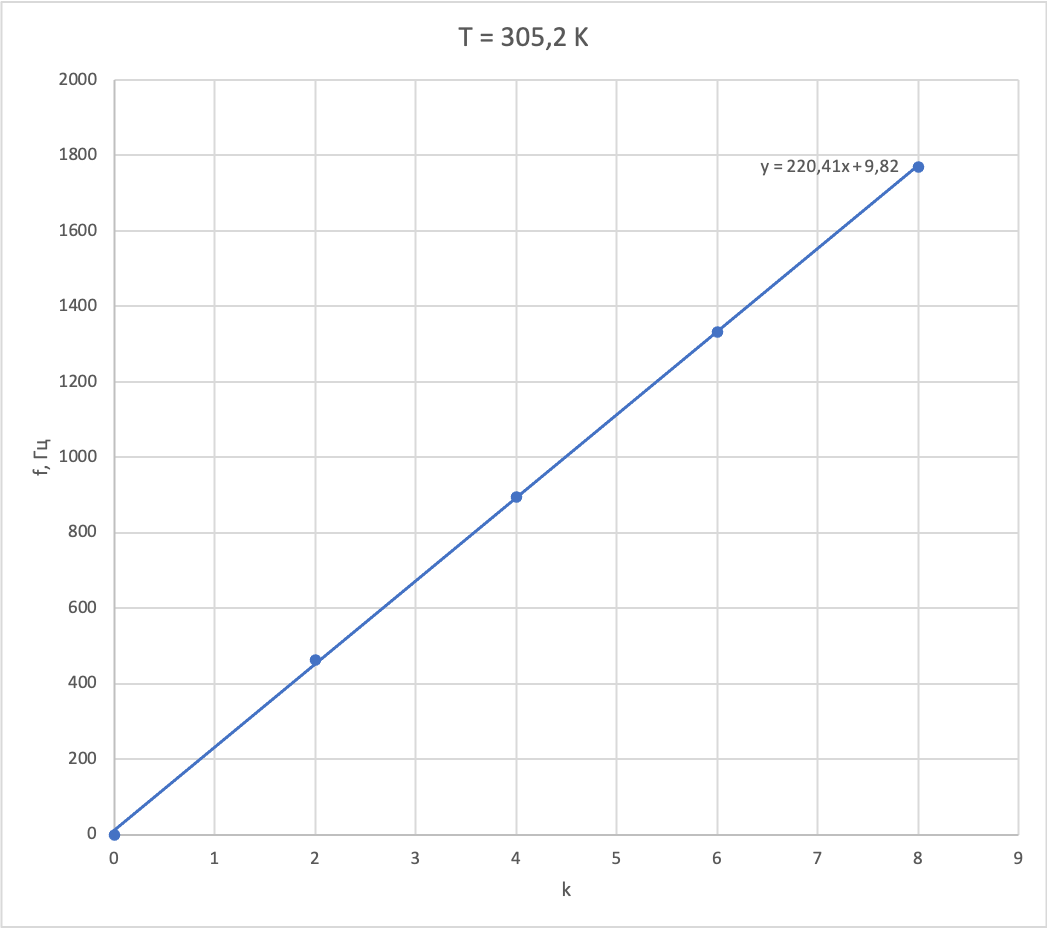
\includegraphics[width=1\linewidth]{5.png}
            \end{minipage}
            \hfill
            \begin{minipage}[h]{0.5\linewidth}
                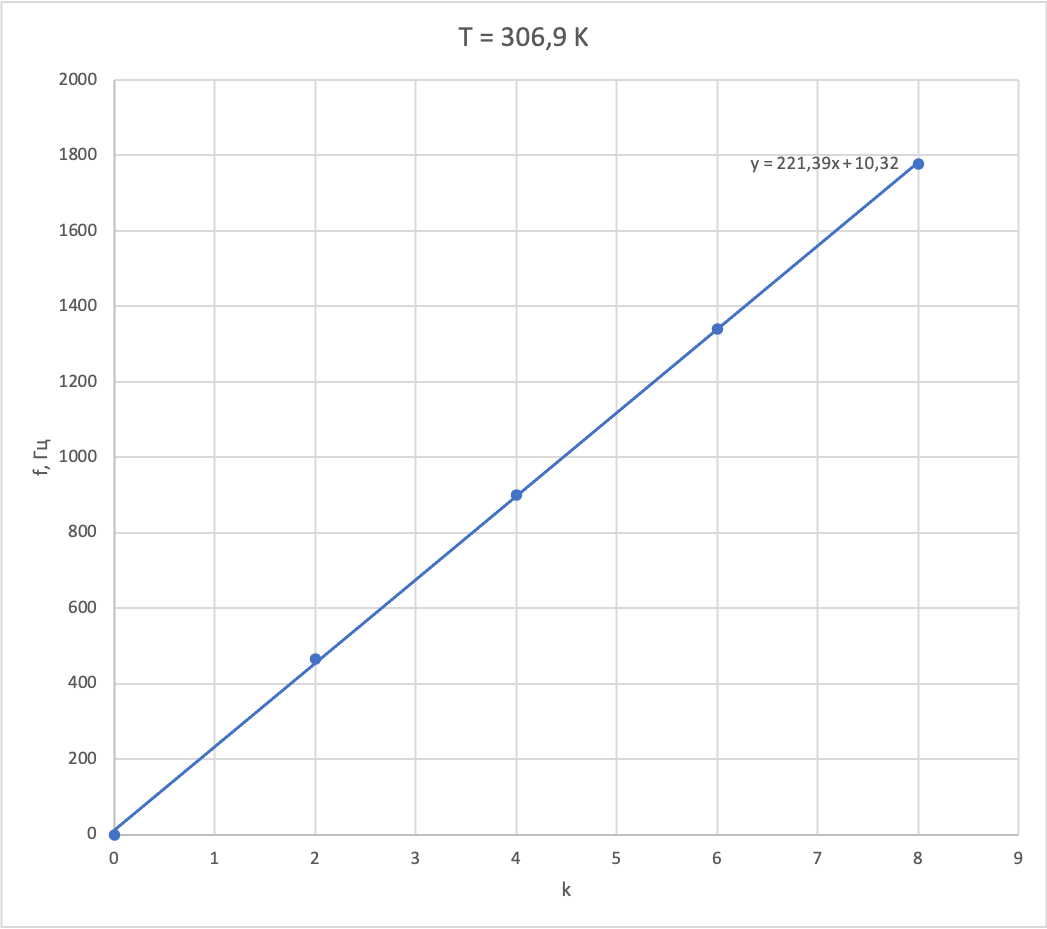
\includegraphics[width=1\linewidth]{6.png}
            \end{minipage}
        \end{figure}
        
        \begin{figure}[ph]
            \begin{minipage}[h]{0.5\linewidth}
                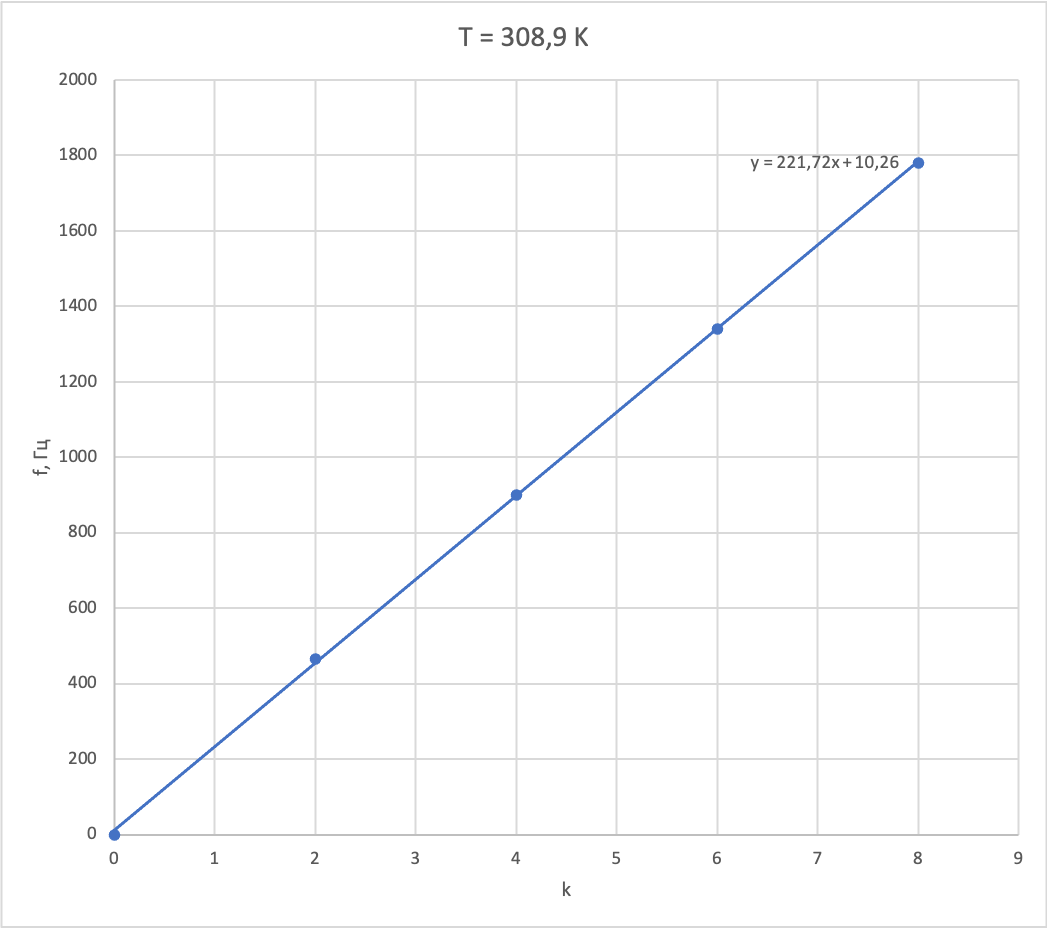
\includegraphics[width=1\linewidth]{7.png}    
            \end{minipage}
            \hfill
            \begin{minipage}[h]{0.5\linewidth}
                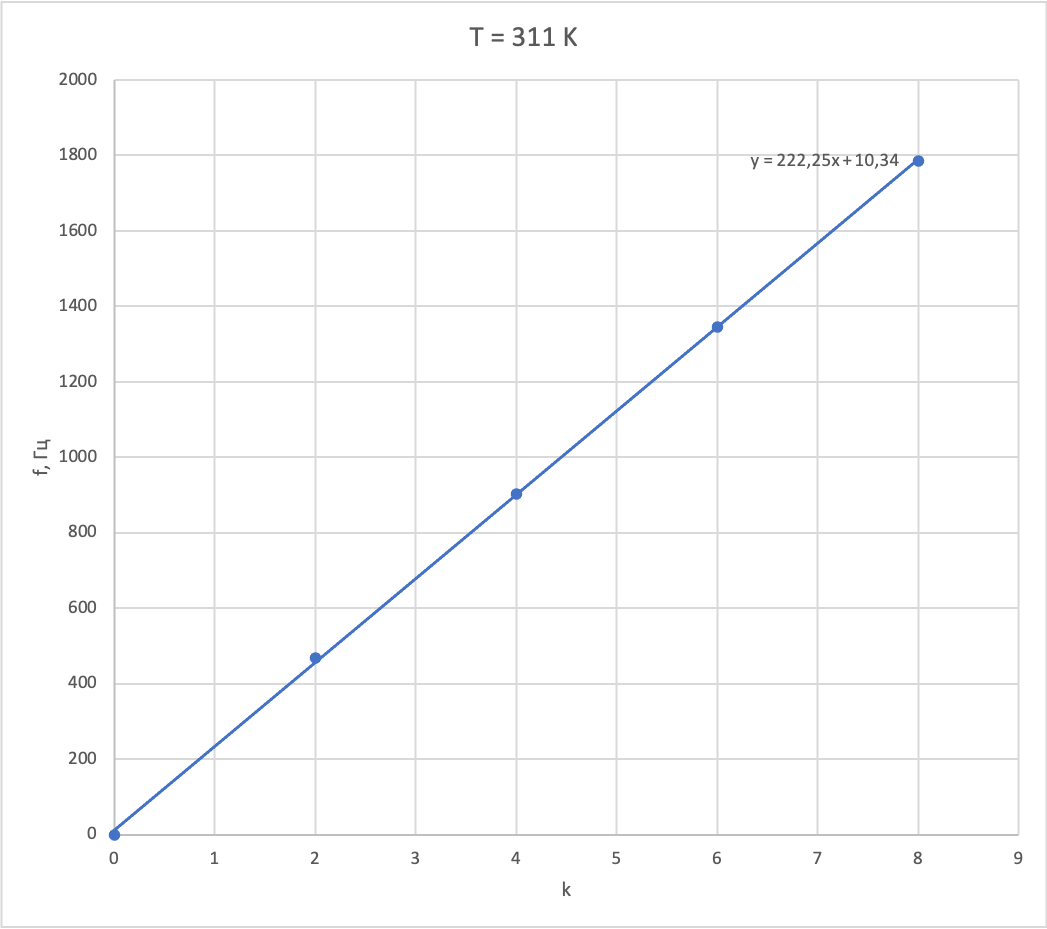
\includegraphics[width=1\linewidth]{8.png}    
            \end{minipage}
            \vfill
            \begin{minipage}[h]{0.5\linewidth}
                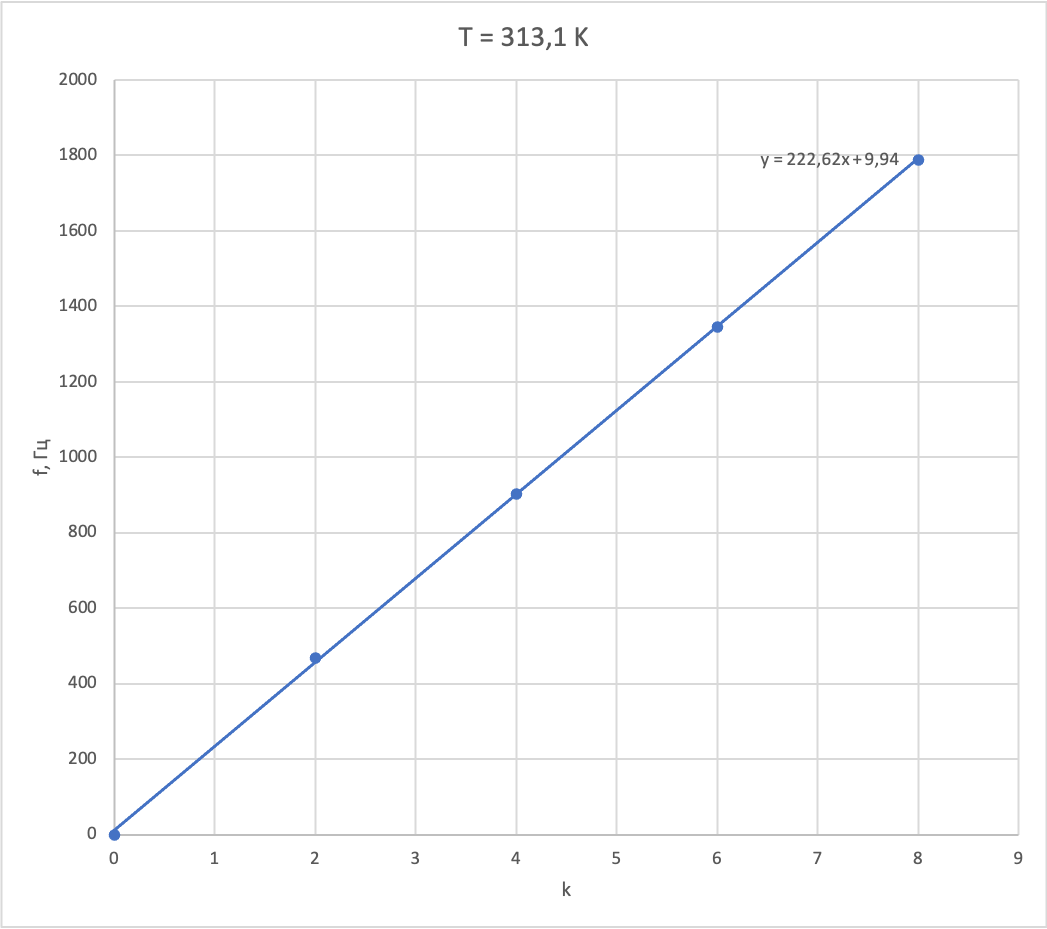
\includegraphics[width=1\linewidth]{9.png}    
            \end{minipage}
            \hfill
            \begin{minipage}[h]{0.5\linewidth}
                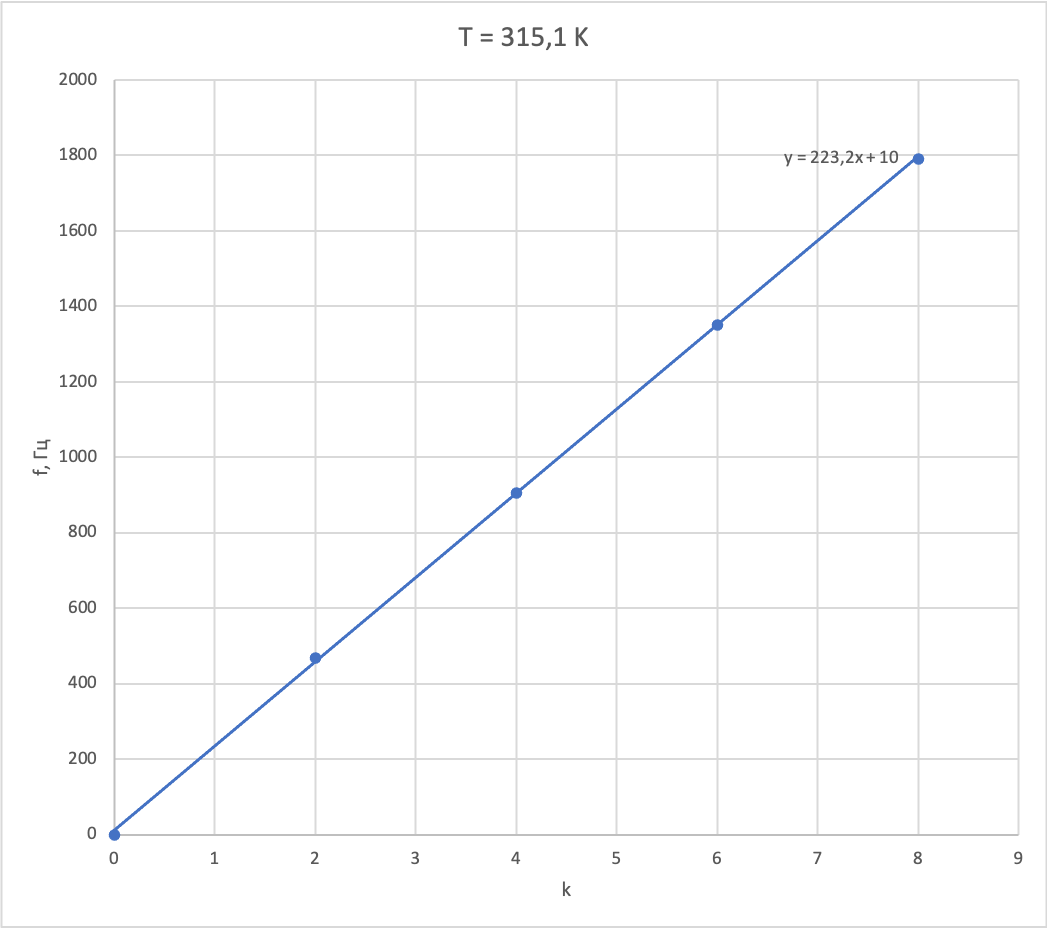
\includegraphics[width=1\linewidth]{10.png}    
            \end{minipage}
            \vfill
            \begin{minipage}[h]{0.5\linewidth}
                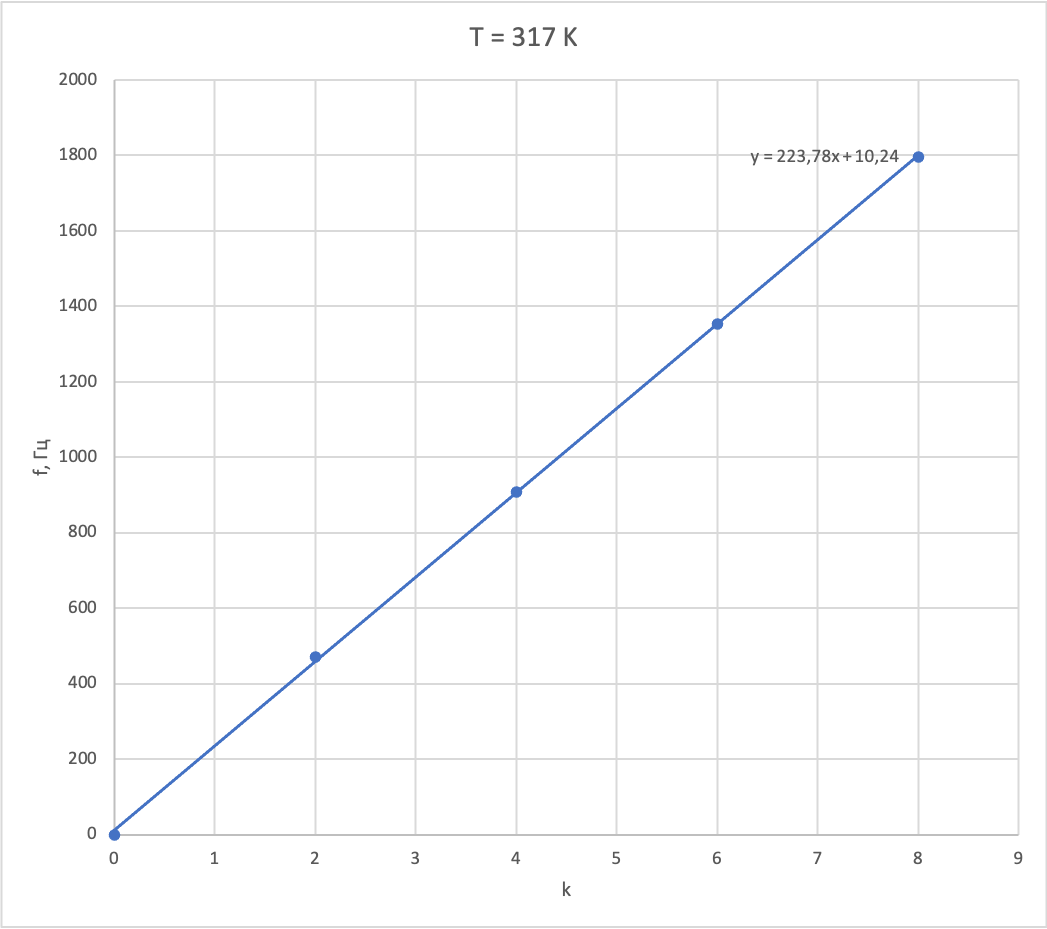
\includegraphics[width=1\linewidth]{11.png}    
            \end{minipage}
            \hfill
            \begin{minipage}[h]{0.5\linewidth}
                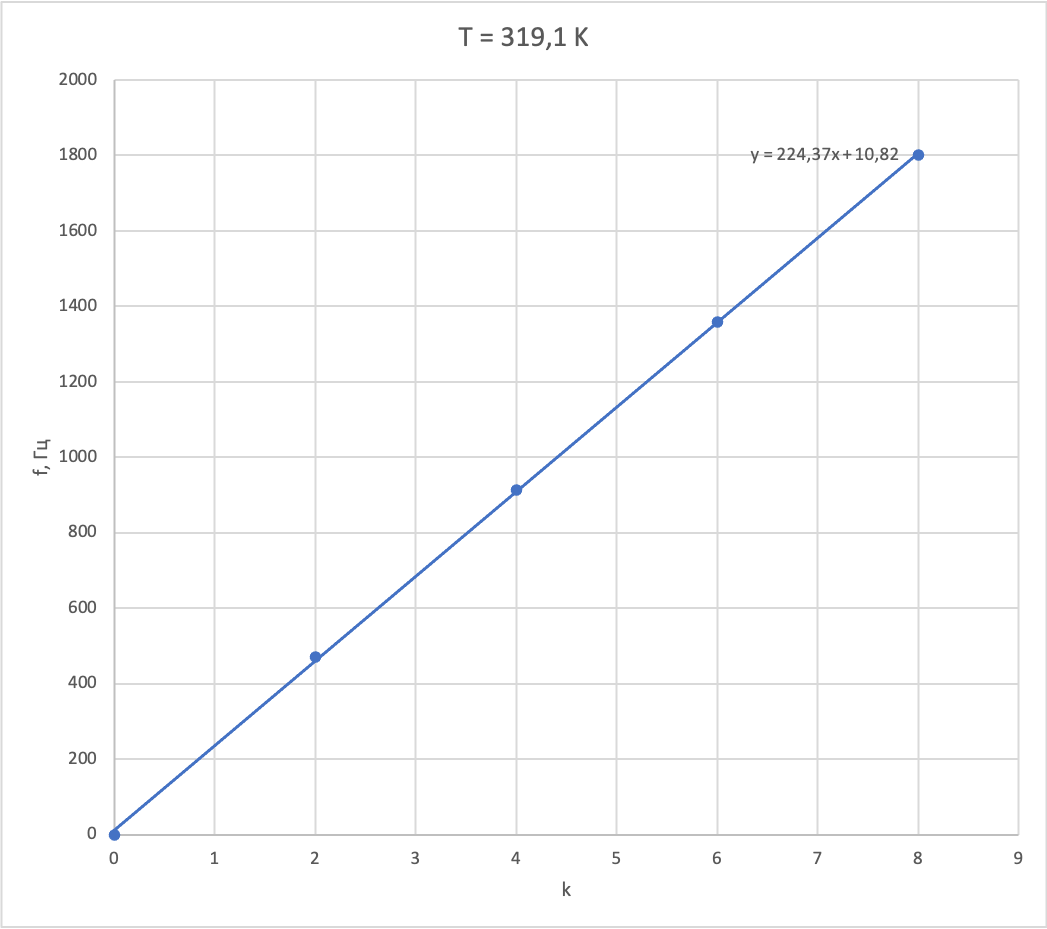
\includegraphics[width=1\linewidth]{12.png}    
            \end{minipage}
        \end{figure}
        
        \begin{figure}[ht]
            \centering
            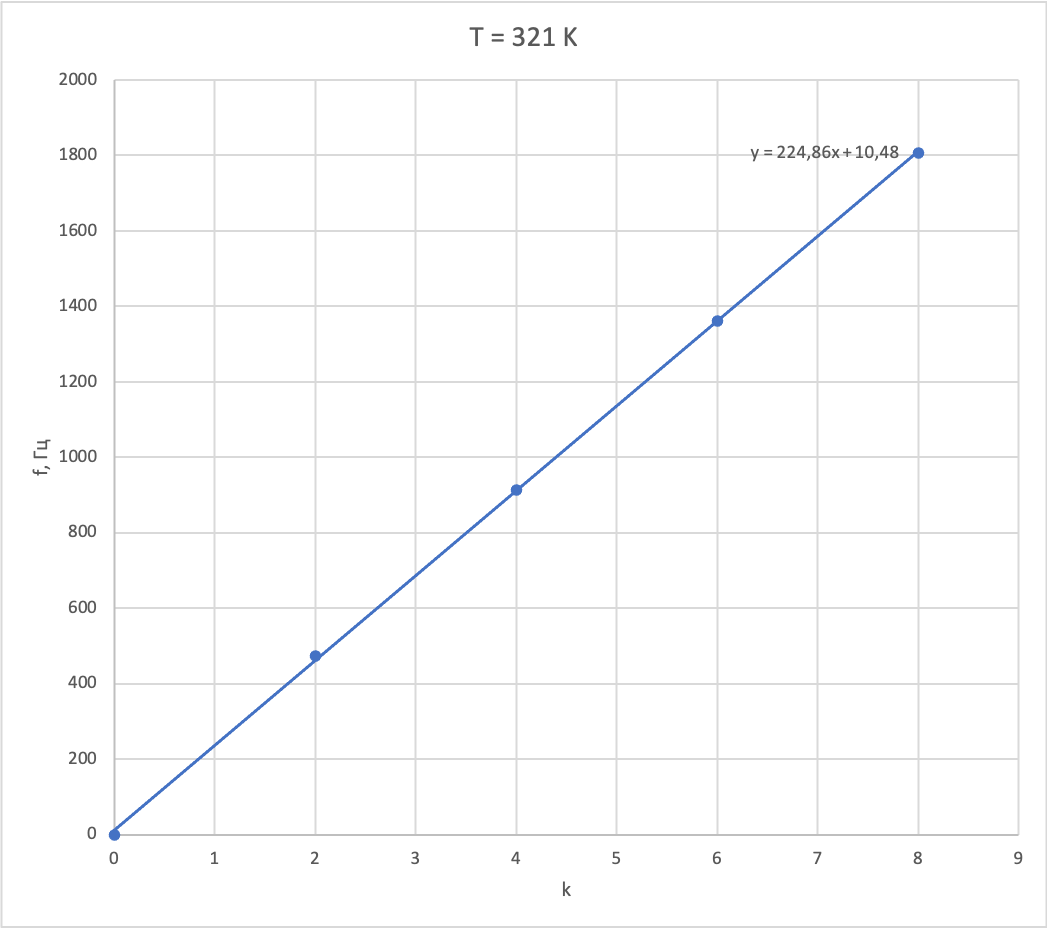
\includegraphics[width=0.5\linewidth]{13.png}
            \caption{Графики зависимостей $f_{k+1} - f_1$ от $k$ при данных температурах $T$}
            \label{pic2}
        \end{figure}
        
        \pagebreak
        
        \item[2.] Зная значения угловых коэффициентов $\alpha$ графиков, представленных на рис. \ref{pic2}, найдём значения скоростей звука: $c = \alpha \cdot 2L$, при данных температурах $T$. Рассчитаем также погрешности каждой величины. Результаты занесём в табл. \ref{table2}.
        
        При подсчёте погрешностей будем пользоваться следующими формулами:
        \begin{equation}
            \varepsilon_{\alpha}^{\text{приб}} = \varepsilon_f,
        \end{equation}
        \begin{equation}
            \varepsilon_c^{\text{случ}} = \varepsilon_{\alpha}^{\text{случ}},
        \end{equation}
        \begin{equation}
            \varepsilon_{\alpha} = \sqrt{(\varepsilon_{\alpha}^{\text{приб}})^2 + (\varepsilon_{\alpha}^{\text{случ}})^2},
        \end{equation}
        \begin{equation}
            \varepsilon_{c}^{\text{приб}} = \sqrt{\varepsilon_{\alpha}^2 + \varepsilon_{L}^2},
        \end{equation}
        \begin{equation}
            \varepsilon_{c} = \sqrt{(\varepsilon_{c}^{\text{приб}})^2 + (\varepsilon_{c}^{\text{случ}})^2}.
        \end{equation}
        
        \begin{table}[ht]
            \centering
            \begin{tabular}{|c|c|c|c|c|c|c|}
                \hline
                $T$, К & $\alpha$, $\text{с}^{-1}$ & $\sigma_{\alpha}$, $\text{с}^{-1}$ & $\varepsilon_{\alpha}$, $\%$ & $c$, м/с & $\sigma_{c}$, м/с & $\varepsilon_c$, $\%$ \\
                \hline
                294,9 & 217,3 & 6,1 & 2,8 & 348 & 10 & 2,8 \\
                \hline
                298 & 218,1 & 6,1 & 2,8 & 349 & 10 & 2,8 \\
                \hline
                300,1 & 219,0 & 6,1 & 2,8 & 350 & 10 & 2,8 \\
                \hline
                302,1 & 219,6 & 6,1 & 2,8 & 351 & 10 & 2,8 \\
                \hline
                305,2 & 220,4 & 6,1 & 2,8 & 353 & 10 & 2,8 \\
                \hline
                306,9 & 221,4 & 6,1 & 2,8 & 354 & 10 & 2,8 \\
                \hline
                308,9 & 221,7 & 6,1 & 2,8 & 355 & 10 & 2,8 \\
                \hline
                311 & 222,3 & 6,1 & 2,8 & 356 & 10 & 2,8 \\
                \hline
                313,1 & 222,6 & 6,1 & 2,7 & 356 & 10 & 2,7 \\
                \hline
                315,1 & 223,2 & 6,1 & 2,7 & 357 & 10 & 2,7 \\
                \hline
                317 & 223,8 & 6,1 & 2,7 & 358 & 10 & 2,7 \\
                \hline
                319,1 & 224,4 & 6,1 & 2,7 & 359 & 10 & 2,7 \\
                \hline
                321 & 224,9 & 6,1 & 2,7 & 360 & 10 & 2,7 \\
                \hline
            \end{tabular}
            \caption{Угловые коэффициенты, скорости звука и их погрешности при данных температурах}
            \label{table2}
        \end{table}
        
        \item[3.] Пользуясь табл. \ref{table2}, запишем квадраты скоростей $c^2$ при данных температурах $T$ в табл. \ref{table3}.
        
        \begin{table}[ht]
            \centering
            \begin{tabular}{|c|c|c|c|c|c|c|c|}
                \hline
                $T$, К & 294,9 & 298 & 300,1 & 302,1 & 305,2 & 306,9 & 308,9 \\ 
                \hline
                $c^2$, $(\text{м/с})^2$ & 121104 & 121801 & 122500 & 123201 & 124609 & 125316 & 126025 \\
                \hline
            \end{tabular}
            \vspace{0.5cm}
            \begin{tabular}{|c|c|c|c|c|c|c|}
                \hline 
                $T$, К & 311 & 313,1 & 315,1 & 317 & 319,1 & 321 \\
                \hline 
                $c^2$, $(\text{м/с})^2$ & 126736 & 126736 & 127449 & 128164 & 128881 & 129600 \\
                \hline
            \end{tabular}
            \caption{Квадраты скоростей $c^2$ при данных температурах $T$}
            \label{table3}
        \end{table}
        
        Проведём наилучшую прямую с помощью МНК через точки зависимости квадратов скоростей звука $c^2$ и температуры $T$, приведённых в табл. \ref{table3}. Результат приведён на рис. \ref{pic3}.
        
        \begin{figure}[ht]
            \centering
            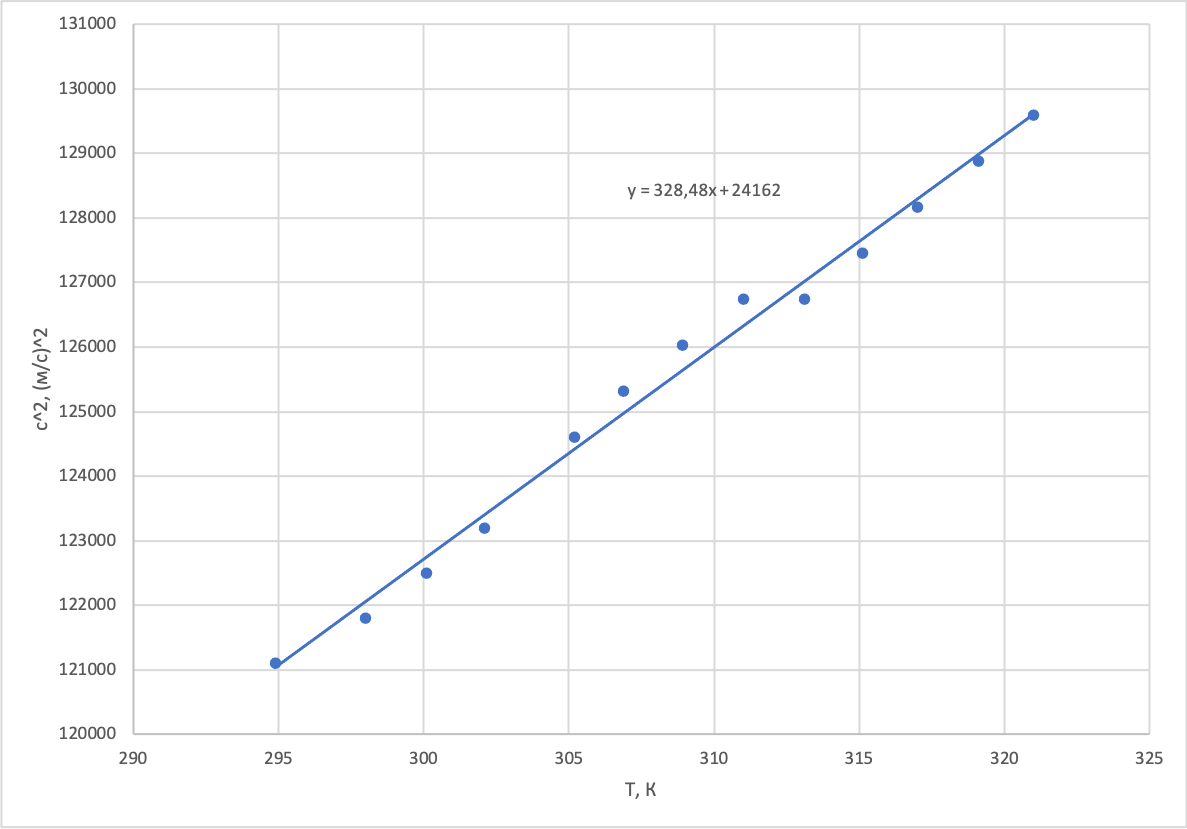
\includegraphics[width=0.8\linewidth]{14.png}
            \caption{График зависимости $c^2$ от $T$}
            \label{pic3}
        \end{figure}
        
        По формуле \eqref{first} видно, что коэффициент наклона этого графика равен: $\beta = \frac{\gamma R}{\mu}$. Тогда: $\gamma = \frac{\beta \mu}{R}$. Зная значения универсальной газовой постоянной: $R = 8,31 \text{ } \frac{\text{м}^2 \cdot \text{кг}}{\text{с}^2 \cdot К \cdot \text{моль}}$, молярной массы воздуха: $\mu_{возд} = 29 \cdot 10^{-3} \text{ } \frac{\text{кг}}{\text{моль}}$, и коэффициента наклона графика: $\beta = 328,5 \text{ } \frac{(\text{м/с})^2}{\text{К}}$, рассчитаем значение показателя адиабаты $\gamma$:
        \begin{equation}
            \gamma = \frac{\beta \mu}{R} = \frac{328,5 \cdot 29 \cdot 10^{-3}}{8,31} = 1,15.
        \end{equation}
        Найдём погрешность данной величины по следующим формулам:
        \begin{equation}
            \varepsilon_{\beta}^{\text{случ}} = 2,6\%,
        \end{equation}
        \begin{equation}
            \varepsilon_{\beta}^{\text{сист}} = \sqrt{4 \cdot \varepsilon_{c}^2 + \varepsilon_{f}^2 + \varepsilon_{T}^2} = 6,4\%,
        \end{equation}
        \begin{equation}
            \varepsilon_{\beta} = \sqrt{(\varepsilon_{\beta}^{\text{случ}})^2 + (\varepsilon_{\beta}^{\text{сист}})^2} = 6,9\%, \text{ } \varepsilon_{\beta} = \varepsilon_{\gamma},
        \end{equation}
        Откуда:
        \begin{equation}
            \gamma = (1,15 \pm 0,08)
        \end{equation}
        
    \end{enumerate}
    
    \begin{flushleft}
        {\Large {\bf Вывод}}
    \end{flushleft}
    
    В ходе данной работы мы сумели определить показатель адиабаты $\gamma$ для воздуха при температурах близких к комнатной ($20^\circ C - 50^\circ C$). Сравнивая полученный результат с табличным ($\gamma_{\text{табл}} \approx 1,3$), можем сказать, что наш результат близок к табличному.
    
\end{document}